\chapter{IMPLEMENTASI}
\tab Pada bab ini akan dipaparkan implementasi dari sistem yang telah dibangun. Bahasa pemrograman yang digunakan adalah bahasa pemrograman Arduino (\textit{Sketch}) yang menyerupai bahasa C untuk memprogram mikrokontroler dan Python untuk menghubungkan mikrokontroler dengan Bot Telegram sebagai pengendali mikrokontrolernya.

\section{Lingkungan Implementasi}
\tab Lingkungan implementasi dalam pembuatan sistem "EasyMeeting" meliputi perangkat keras dan perangkat lunak yang digunakan untuk mengimplementasikan sistem yang telah dirancang adalah sebagai berikut:
\begin{enumerate}
	\item Perangkat Keras
	\begin{itemize}
		\item Komponen Mikrokontroler
		\begin{itemize}
			\item Arduino UNO
			\item DHT11
			\item \textit{Breadboard}
			\item Resistor
			\item \textit{Jumper Wires}
			\item Lampu LED
			\item \textit{Infrared Sensor Module}
			\item \textit{Infrared Receiver Module}
		\end{itemize}
		\item Laptop
		\begin{itemize}
			\item \textit{Processor} Intel(R) Core(TM) i7-4510U CPU @ 2.00GHz
			\item Memori 4 GB (3,92514 GB)
		\end{itemize}
	\end{itemize}
	\item Perangkat Lunak
	\begin{itemize}
		\item Sistem Operasi Linux (Linux Mint 18.3 Sylvia)
		 64-bit
		\item \textit{Text Editor} Visual Studio Code
		\item \textit{Software} Arduino IDE
		\item Bahasa Pemrograman C/C++
		\item \textit{Version Control System} Git
	\end{itemize}
\end{enumerate}

\section{Implementasi Rangkaian Mikrokontroler}
\tab Pada bagian ini akan dijelaskan mengenai implementasi rangkaian mikrokontroler pada sistem EasyMeeting. Untuk pengimplementasiannya, dibutuhkan beberapa komponen mikrokontroler yaitu:
\begin{enumerate}
	\item Arduino UNO
	\begin{figure}[H]
		\centerline {
			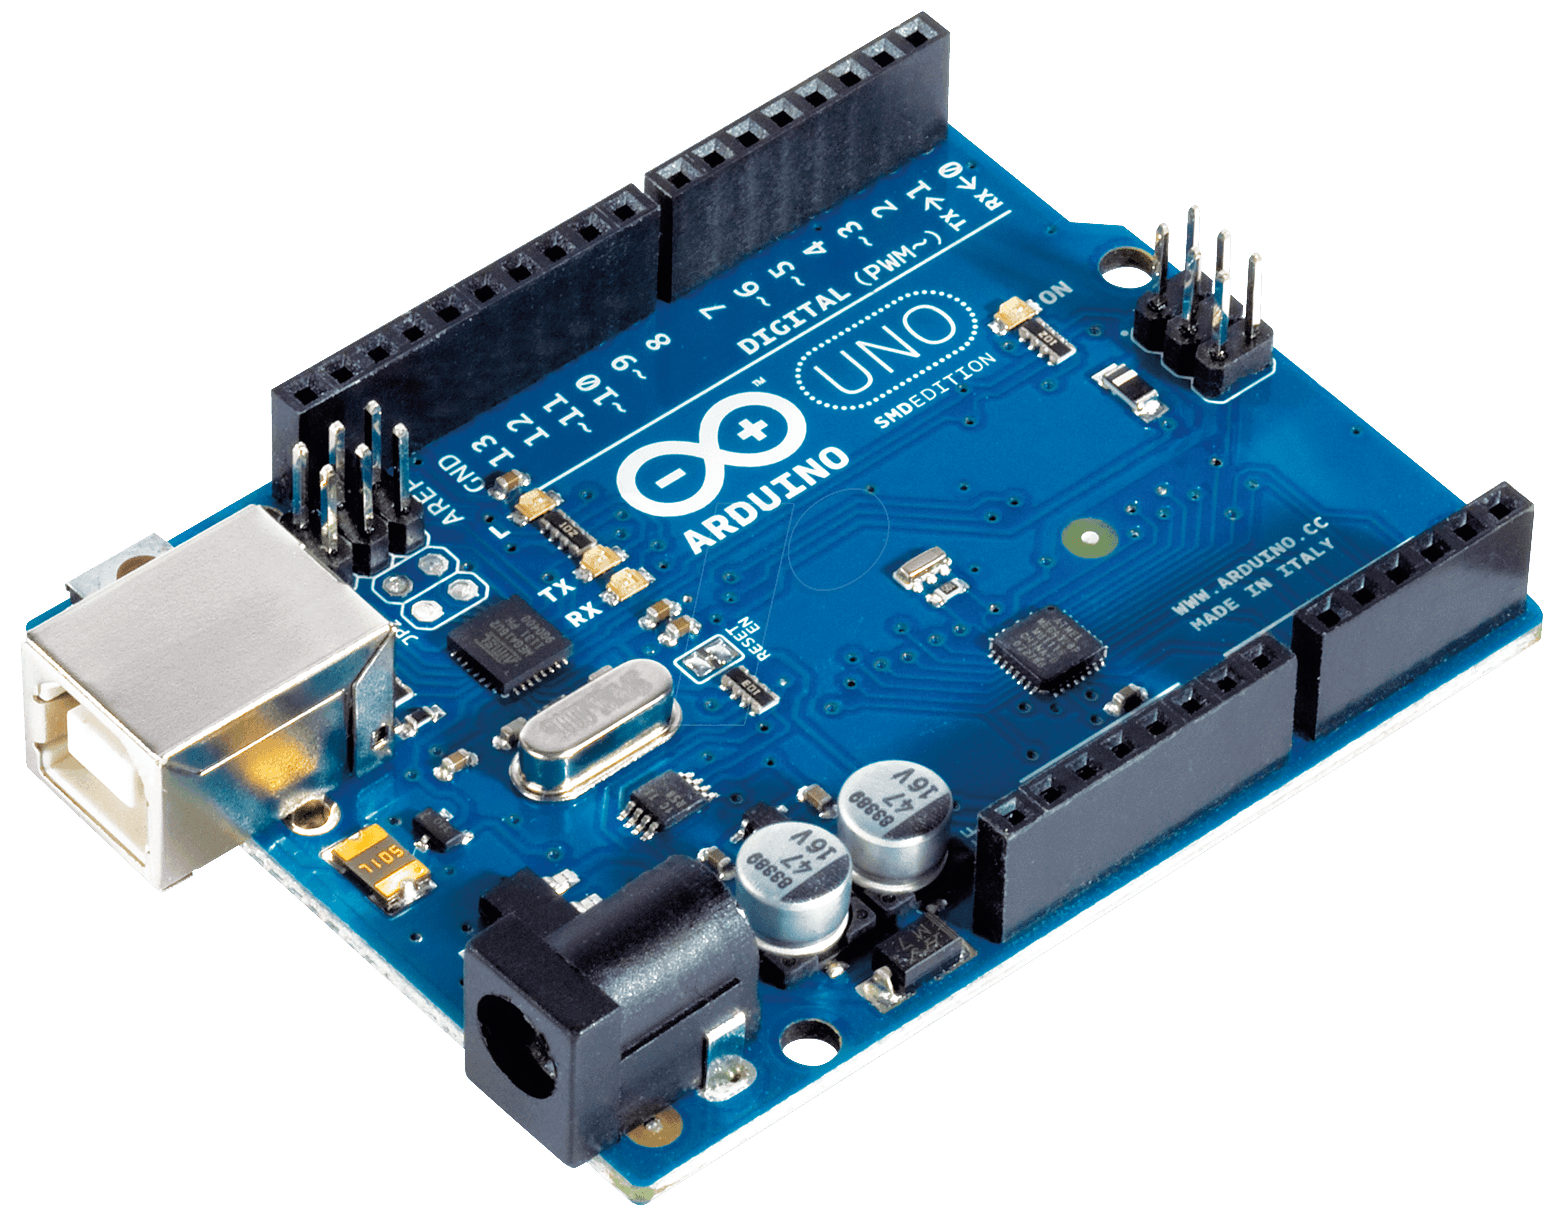
\includegraphics[width=10cm,height=7.5cm]{bab5/img/ARDUINO.png}
		}
		\caption{Arduino UNO}
		\label{figure:arduino}
	\end{figure}
	\tab Arduino Uno adalah board mikrokontroler berbasis ATmega328 (datasheet). Memiliki 14 pin input dari output digital  dimana 6 pin input tersebut dapat digunakan sebagai output PWM dan 6 pin input analog, 16 MHz osilator kristal, koneksi USB, jack power, ICSP header, dan tombol reset. Untuk mendukung mikrokontroler agar dapat digunakan, cukup hanya menghubungkan Board Arduino Uno ke komputer dengan menggunakan kabel USB atau listrik dengan AC yang-ke adaptor-DC atau baterai untuk menjalankannya.
	\pagebreak
	\item DHT11
	\begin{figure}[H]
		\centerline {
			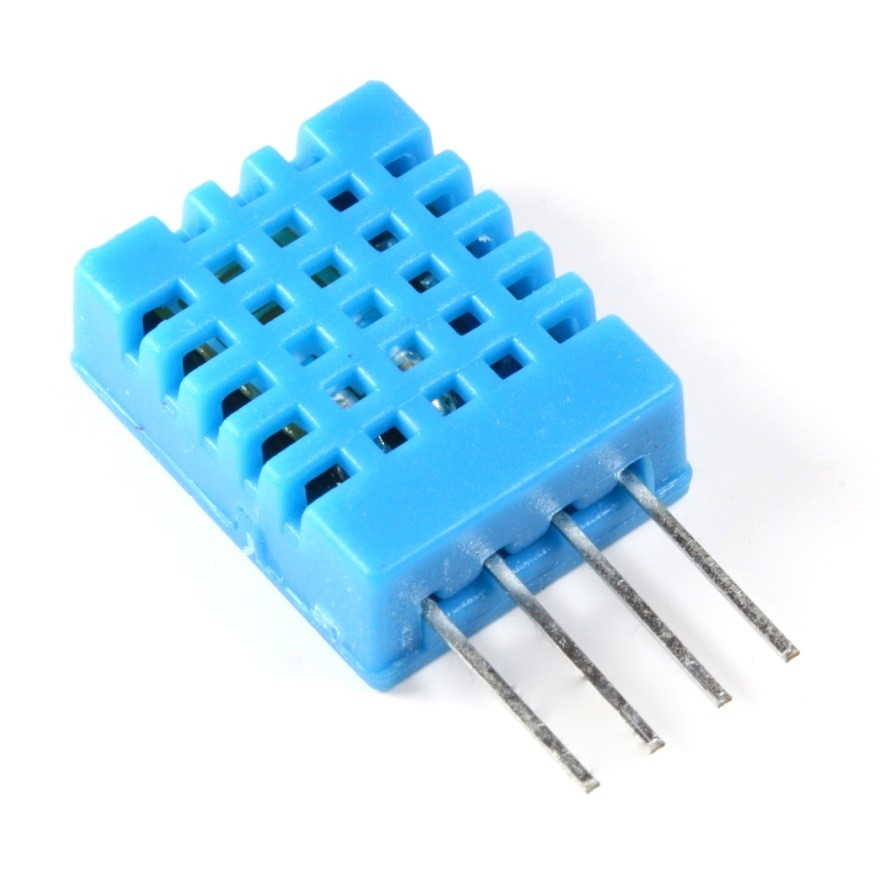
\includegraphics[width=10cm,height=7.5cm]{bab5/img/dht11.png}
		}
		\caption{Sensor Suhu DHT11}
		\label{figure:dth11}
	\end{figure}
	\tab DHT11 adalah sensor suhu dan kelembaban. Ia memiliki keluaran sinyal digital yang dikalibrasi dengan sensor suhu dan kelembaban yang kompleks. Teknologi ini memiliki tingkat keakuratan tinggi dan stabilitas yang baik untuk penggunaan jangka panjang.
	\pagebreak
	\item \textit{Breadboard}
	\begin{figure}[H]
		\centerline {
			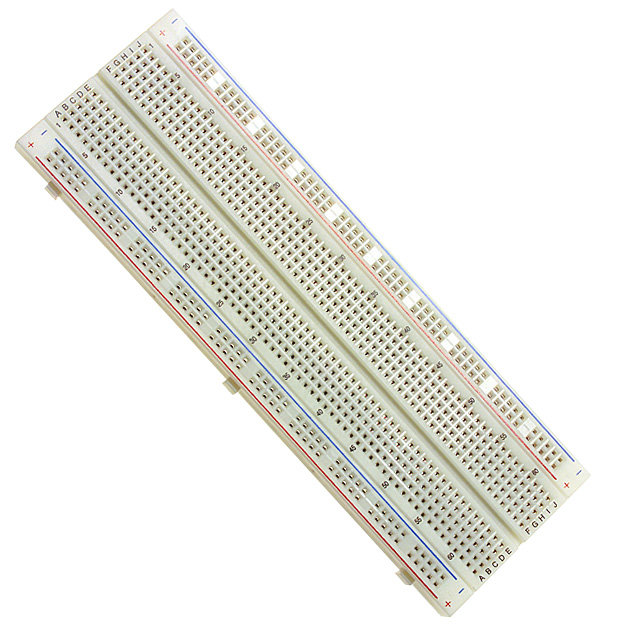
\includegraphics[width=10cm,height=7.5cm]{bab5/img/breadboard.png}
		}
		\caption{\textit{Breadboard}}
		\label{figure:breadboard}
	\end{figure}
	\tab \textit{Breadboard} merupakan sebuah sirkuit elektronik dan merupakan prototipe dari suatu rangkaian elektronik. Bentuk \textit{Breadboard} tertera pada Gambar \ref{figure:breadboard}.
	\pagebreak
	\item Resistor
	\begin{figure}[H]
		\centerline {
			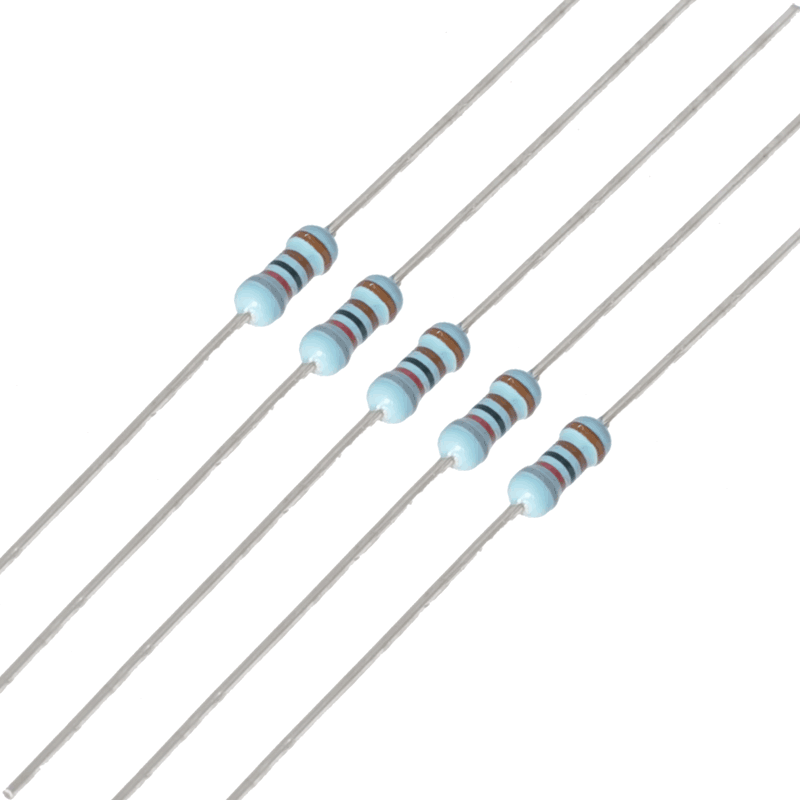
\includegraphics[width=10cm,height=7.5cm]{bab5/img/resistor.png}
		}
		\caption{Resistor}
		\label{figure:resistor}
	\end{figure}
	\tab Resistor merupakan penghambat arus listrik agar bisa menyesuaikan kebutuhan perangkat keras agar tidak terjadi kerusakan pada peralatan mikrokontroler saat dialirkan tegangan listrik. Terdapat banyak resistor yang bisa didapatkan berdasarkan besar hambatannya. Banyaknya garis dan perbedaan warna pada resistor menunjukan perbedaan tegangan. Bentuk resistor dapat dilihat pada Gambar \ref{figure:resistor}.
	\pagebreak
	\item \textit{Jumper Wires}
	\begin{figure}[H]
		\centerline {
			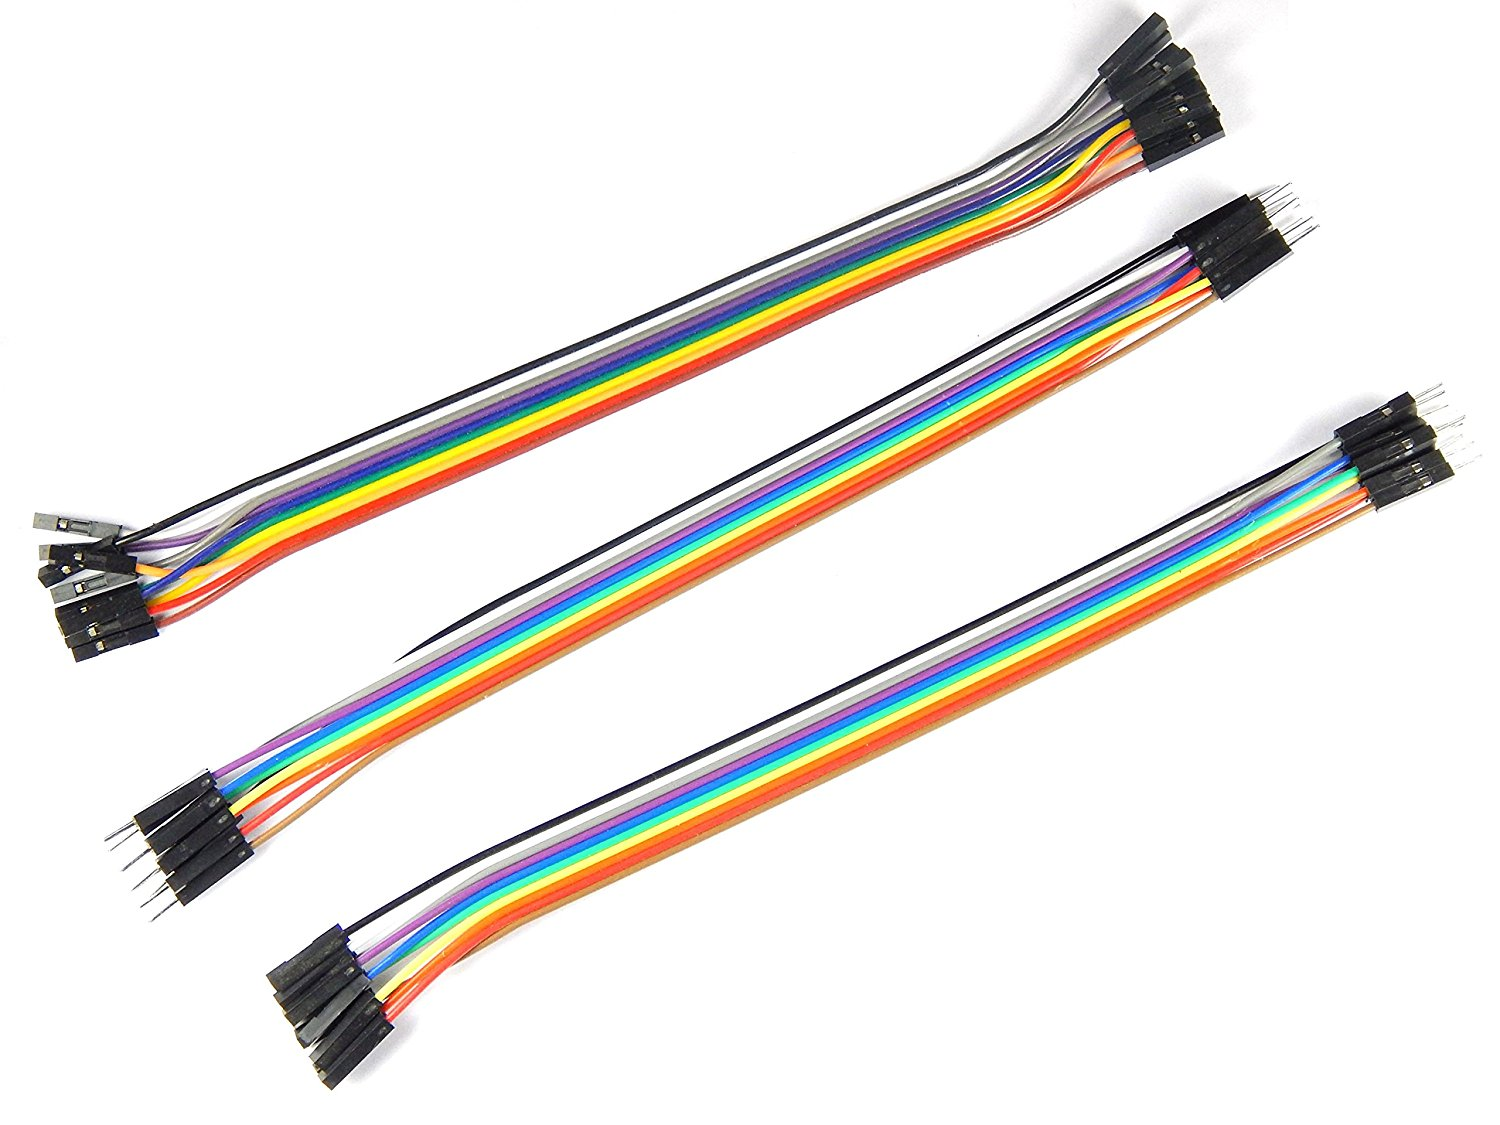
\includegraphics[width=10cm,height=7.5cm]{bab5/img/jumper.png}
		}
		\caption{\textit{Jumper Wires}}
		\label{figure:jumper}
	\end{figure}
	\tab Jumper adalah sebuah konektor sirkuit elektrik yang digunakan untuk menghubungkan atau memutuskan hubungan pada suatu sirkuit. Bentuk jumper dapa dilihat pada Gambar \ref{figure:jumper}.
	\pagebreak
	\item Lampu LED
	\begin{figure}[H]
		\centerline {
			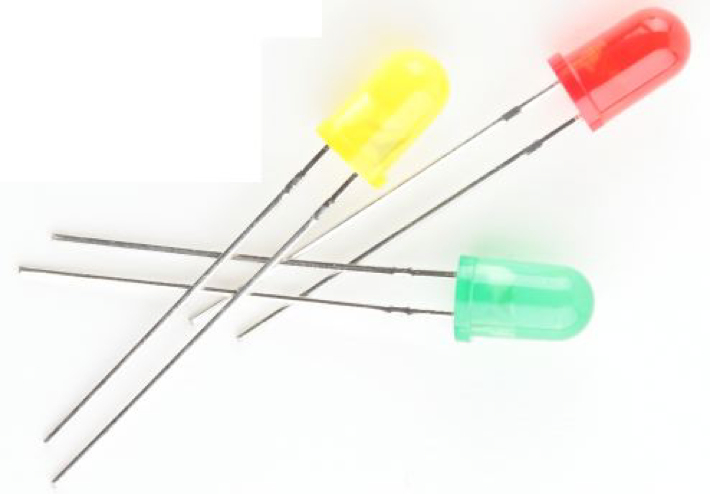
\includegraphics[width=10cm,height=7.5cm]{bab5/img/led.png}
		}
		\caption{Lampu LED}
		\label{figure:led}
	\end{figure}
	\tab Lampu LED digunakan sebagai prototipe dari lampu ruangan. Lampu LED akan menyala ketika perintah untuk menyalakan lampu dijalankan. Lampu LED yang kami gunakan berukuran 5 mm. Gambar Lampu LED tertera pada Gambar \ref{figure:led}.
	\pagebreak
	\item \textit{Infrared Transmitter Module}
	\begin{figure}[H]
		\centerline {
			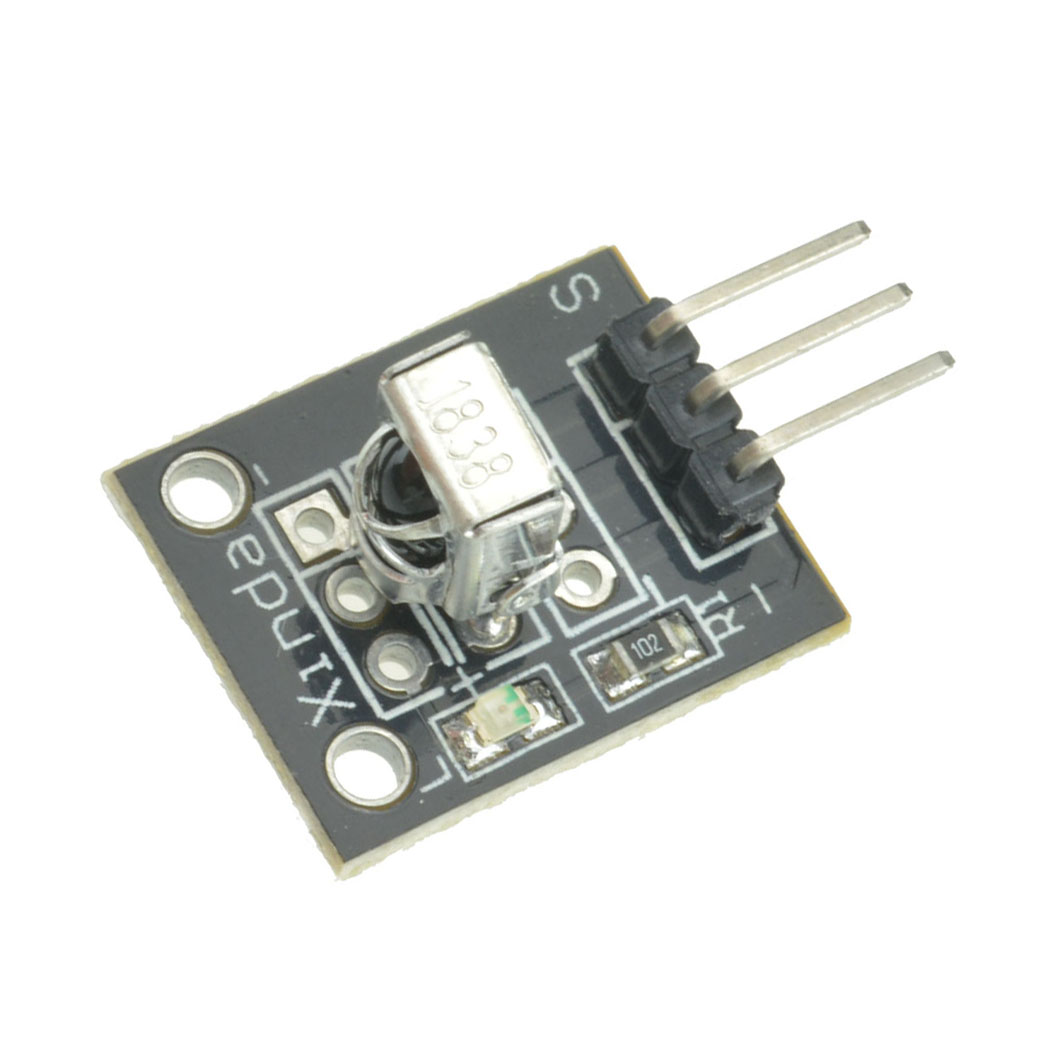
\includegraphics[width=10cm,height=7.5cm]{bab5/img/transmitter.png}
		}
		\caption{\textit{Infrared Transmitter Module}}
		\label{figure:transmitter}
	\end{figure}
	\tab \textit{Infrared Transmitter Module} digunakan untuk memberikan sinyal Infrared ke AC yang berada dalam ruang rapat untuk menyalakan dan mematikan AC dalam ruangan tersebut. Gambar \textit{Infrared Transmitter Module} tertera pada Gambar \ref{figure:transmitter}.
	\pagebreak
	\item \textit{Infrared Receiver Module}
	\begin{figure}[H]
		\centerline {
			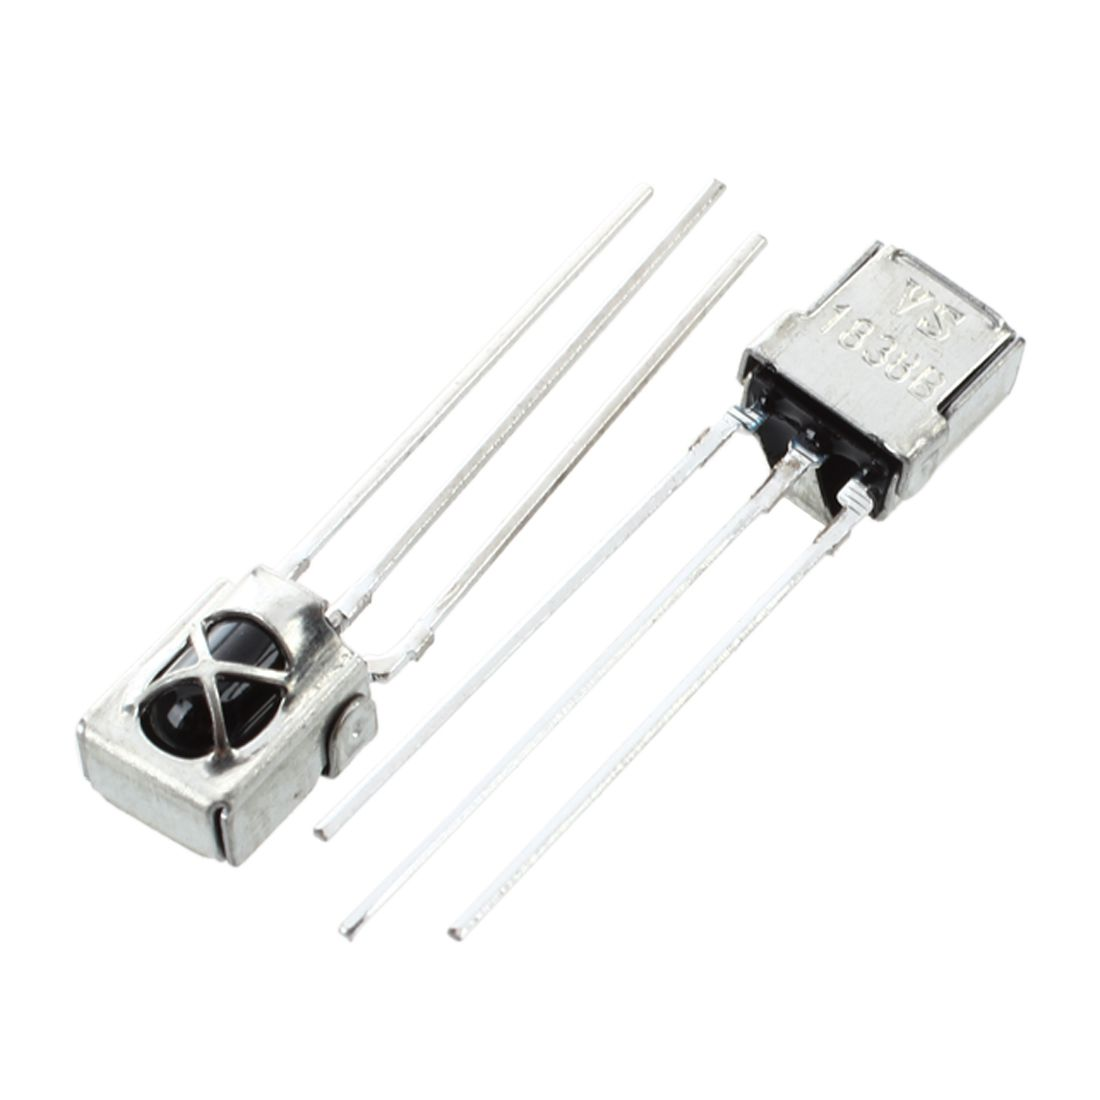
\includegraphics[width=10cm,height=7.5cm]{bab5/img/receiver.png}
		}
		\caption{\textit{Infrared Receiver Module}}
		\label{figure:receiver}
	\end{figure}
	\tab \textit{Infrared Receiver Module} digunakan untuk membaca kode pada tombol remot AC yang berada di dalam ruang rapat agar \textit{Infrared Transmitter Module} dapat mengendalikan AC seesuai dengan perintah yang dijalankan pada Arduino. Gambar \textit{Infrared Transmitter Module} tertera pada Gambar \ref{figure:receiver}.
\end{enumerate}
\pagebreak
Semua komponen di atas kemudian dirangkai menjadi satu kesatuan sesuai dengan perancangan sistem. Langkah-langkah yang dilakukan adalah:
\begin{enumerate}
	\item Buat sirkuit Mikrokontroler Arduino UNO dengan Modul WiFi ESP8266-01 agar dapat terhubung dengan \textit{access point} WiFi.
	\begin{figure}[H]
		\centerline {
			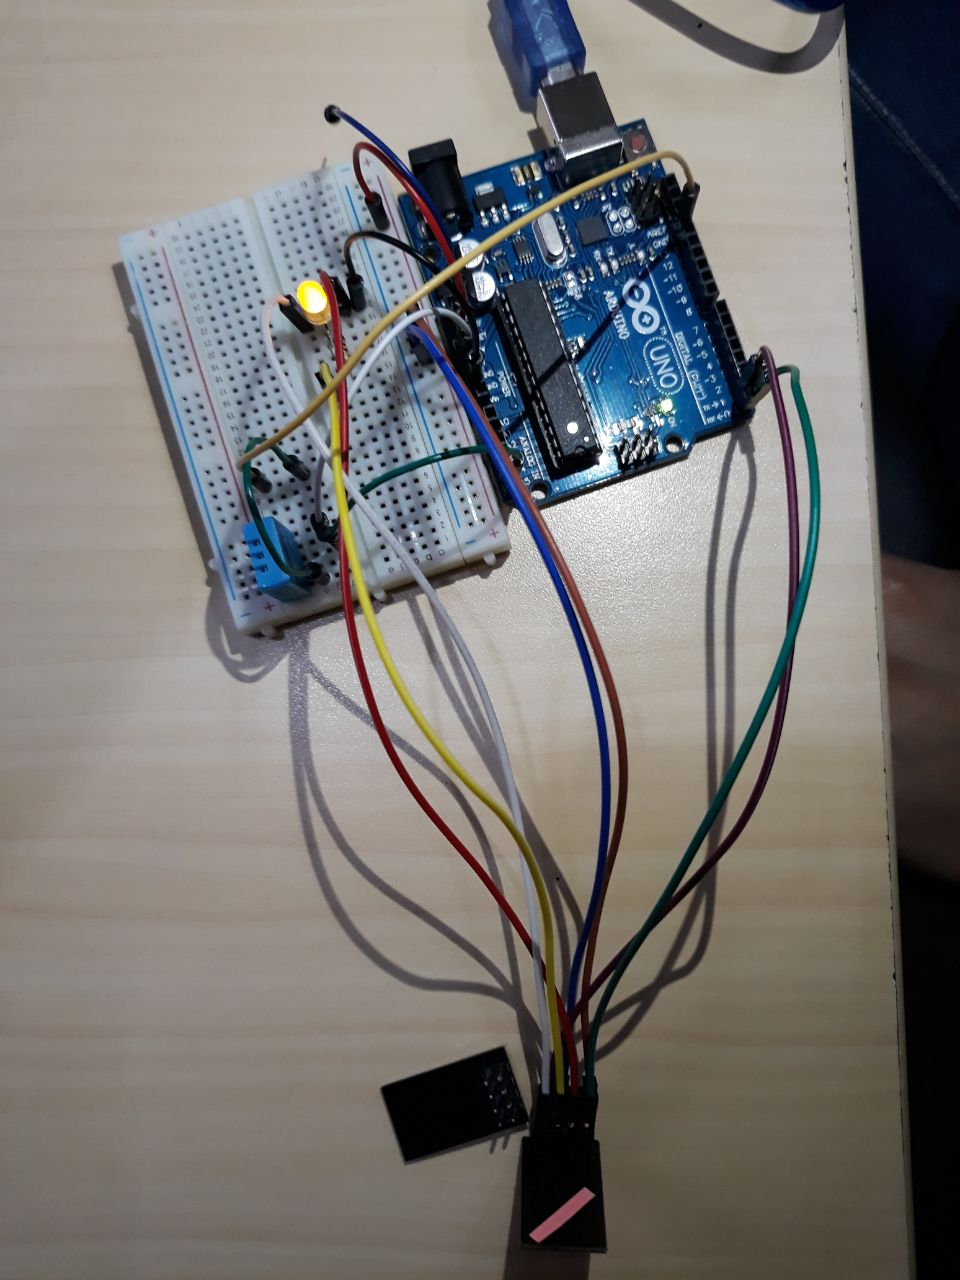
\includegraphics[width=6cm]{bab5/img/wifi.jpeg}
		}
		\caption{Sirkuit untuk ESP8266-01 WiFi Module}
		\label{figure:wifi}
	\end{figure}
	\item Buat sirkuit untuk menghubungkan sensor DHT11, \textit{Infrared Transmitter Module}, dan lampu LED dengan Mikrokontroler Arduino UNO.
	\begin{figure}[H]
		\centerline {
			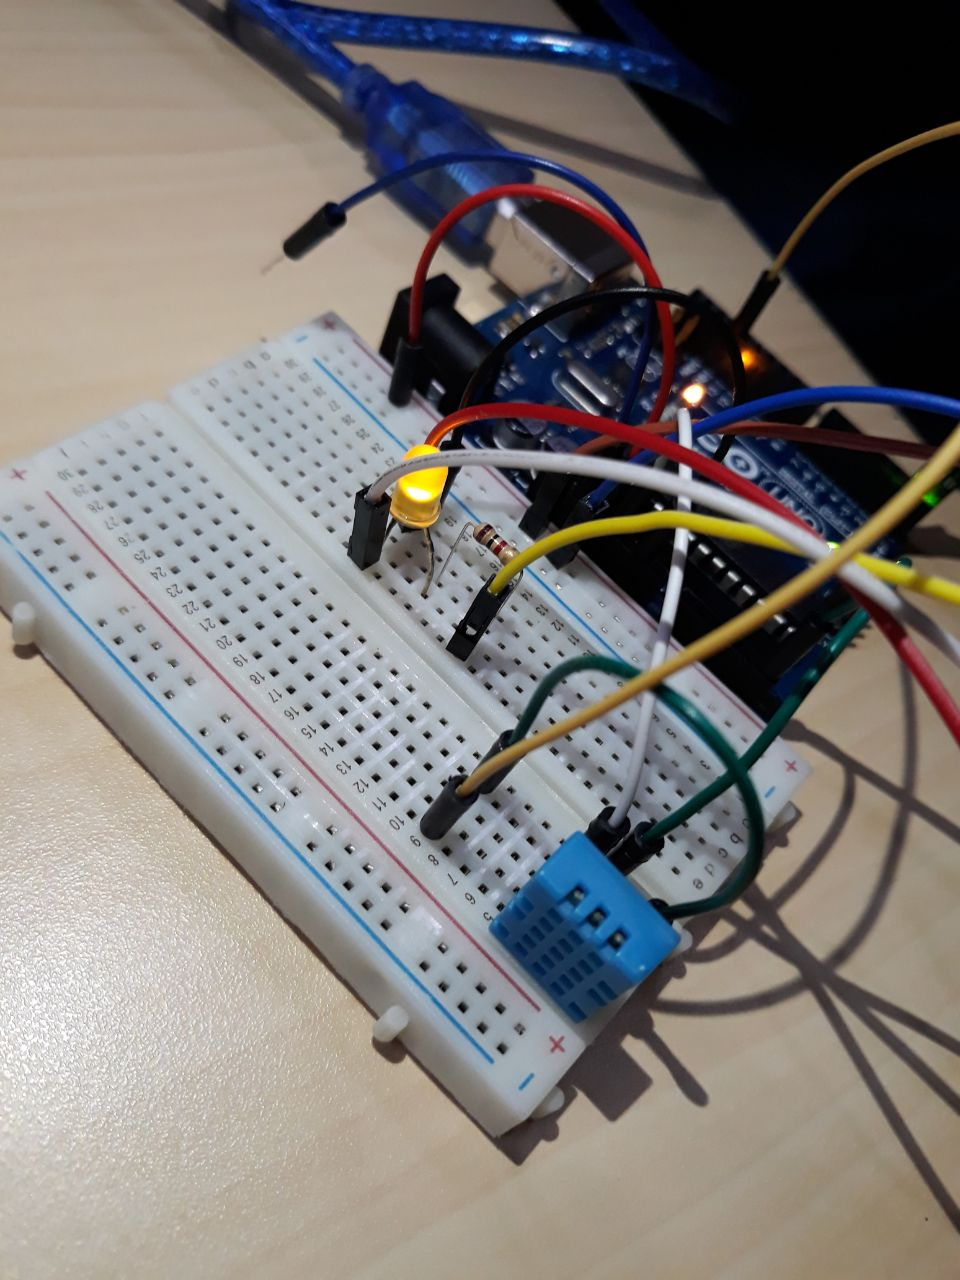
\includegraphics[width=6cm]{bab5/img/sensor.jpeg}
		}
		\caption{Sirkuit untuk Keseluruhan Modul Mikrokontroler yang digunakan}
		\label{figure:sensor}
	\end{figure}
\end{enumerate}

\section{Implementasi Lapisan Kontrol Sistem}
\tab Pada bagian ini akan dijelaskan mengenai lapisan kontrol sistem yang berfungsi untuk mengontrol keseluruhan sistem EasyMeeting, meliputi kontrol mikrokontroler hingga menghubungkan mikrokontroler dengan antarmuka pengguna (Bot API Telegram). Lapisan kontrol sistem dibuat menggunakan bahasa pemrograman C/C++ yang untuk menjalankan Bot API Telegram pada Arduino Uno.

\subsection{Menghubungkan Mikrokontroler dengan WiFi}
\tab Mikrokontroler yang telah dirangkai harus tersambung dengan internet agar dapat menjankan Bot pada aplikasi Telegram. Untuk menghubungkan Arduino ke WiFi pada Hotspot area di PT. Telekomunikasi Indonesia dapat dihubungkan melalui sistem Arduino tersebut.
\lstinputlisting[language=C++, firstline=6, lastline=7, caption=Potongan Kode untuk Menghubungkan Koneksi Arduino ke WiFi, label={lst:wifi}]{bab5/src/led.ino}

\subsection{Menghubungkan Mikrokontroler dengan Bot Telegram}
Bot EasyMeeting pada aplikasi Telegram akan berjalan ketika sistem (Mikrokontroler) yang berperan sebagai \textit{server} terhubung ke Telegram dengan API.
\lstinputlisting[language=C++, firstline=10, lastline=14, caption=Potongan Kode untuk Menghubungkan Arduino ke Bot Telegram, label={lst:bot}]{bab5/src/led.ino}

\section{Implementasi Antarmuka Pengguna}
\tab Pada bagian ini akan dijelaskan mengenai bagaimana pengguna dapat berinteraksi dengan sistem EasyMeeting melalui platform Telegram. Telegram menyediakan dua jenis API yang dapat dikembangkan bebas oleh pengguna, yakni Telegram API dan Bot API. Penulis memanfaatkan Bot API Telegram untuk membuat antarmuka sistem berupa \textit{chat bot} yang dapat berinteraksi dengan pengguna. Langkah-langkah yang dilakukan untuk membuat Bot API Telegram yaitu:
\begin{enumerate}
	\item Mengirimkan permintaan kepada "BotFather" Telegram untuk mendapatkan API Bot yang akan digunakan. Cara untuk membuat Bot pada aplikasi Telegram dapat dilihat pada Gambar \ref{figure:newbot}.
	\begin{figure}[H]
		\centerline {
			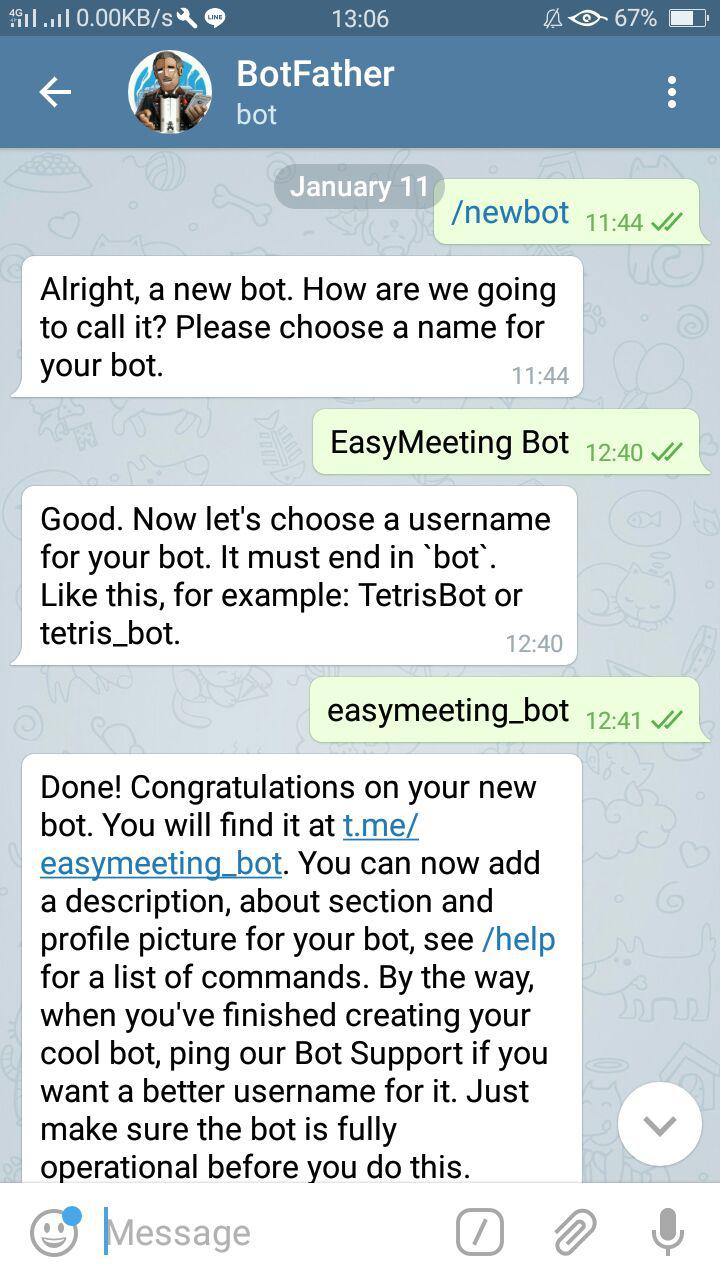
\includegraphics[width=3.5cm]{bab5/img/newbot.jpg}
		}
		\caption{Membuat EasyMeeting Bot sebagai Bot baru pada aplikasi Telegram}
		\label{figure:newbot}
	\end{figure}
	\item "BotFather" Telegram akan mengirimkan API untuk dapat menjalankan  Bot pada Telegram agar dapat digunakan pada sistem yang akan dibuat.
	\begin{figure}[H]
		\centerline {
			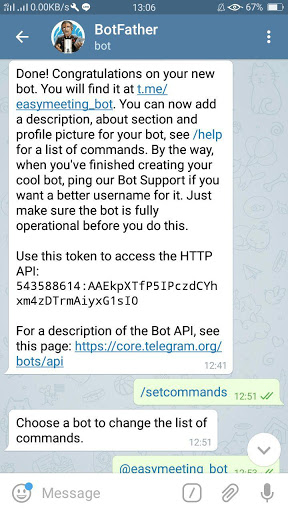
\includegraphics[width=3cm]{bab5/img/api.jpg}
		}
		\caption{"BotFather" Telegram mengirimkan API dari Bot yang baru dibuat}
		\label{figure:api}
	\end{figure}
	\item Perintah dapat langsung dibuat melalui "BotFather" Telegram dengan mengirimkan perintah "/setcommands". Cara untuk menambahkan perintah pada Bot yang dimiliki dapat dilihat pada Gambar \ref{figure:cmd}.
	\begin{figure}[H]
		\centerline {
			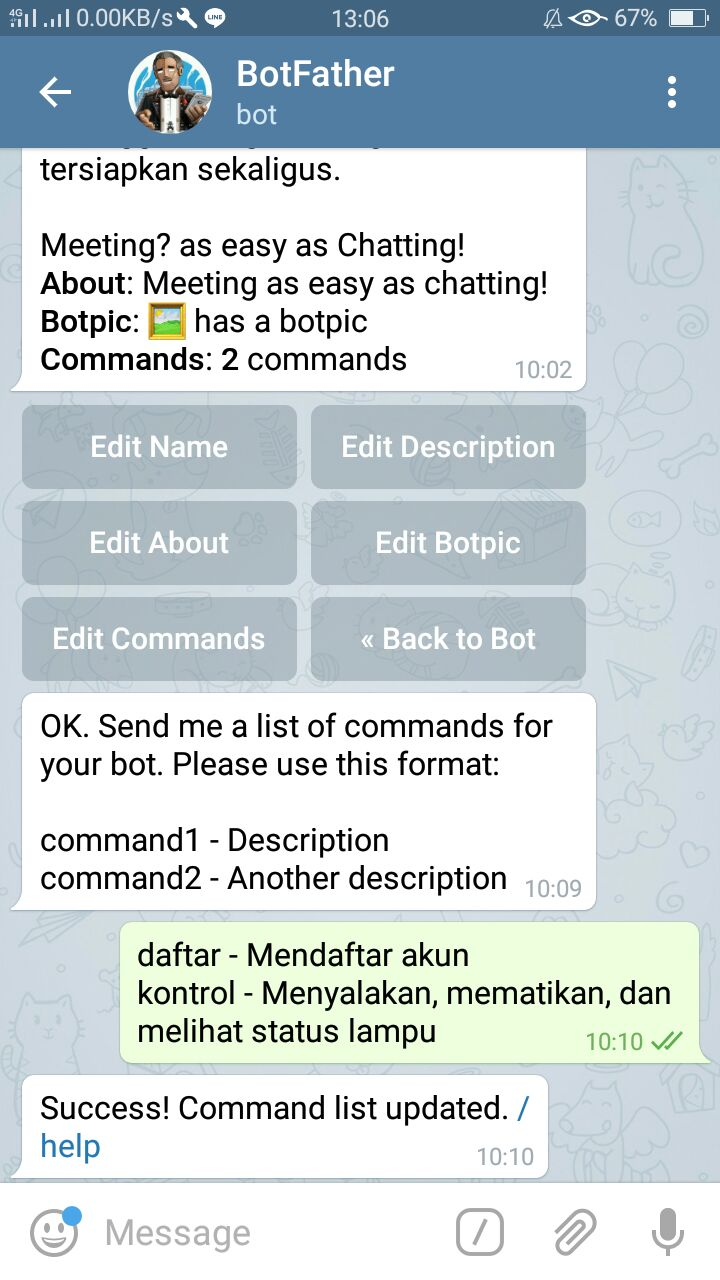
\includegraphics[width=3cm]{bab5/img/cmd.jpeg}
		}
		\caption{Menambahkan perintah pada Bot sesuai dengan kebutuhan}
		\label{figure:cmd}
	\end{figure}
\end{enumerate}

\subsection{Tampilan Menu Perintah dengan GUI}
\lstinputlisting[language=C++, firstline=58, lastline=64, caption=Potongan Kode untuk Menampilkan Menu Perintah, label={lst:menu}]{bab5/src/led.ino}

\subsection{Menyalakan Lampu dan AC Ruangan}
\lstinputlisting[language=C++, firstline=32, lastline=38, caption=Potongan Kode untuk Menyalakan Lampu dan AC, label={lst:nyalakan}]{bab5/src/led.ino}

\subsection{Mematikan Lampu dan AC Ruangan}
\lstinputlisting[language=C++, firstline=40, lastline=46, caption=Potongan Kode untuk Mematikan Lampu dan AC, label={lst:matikan}]{bab5/src/led.ino}
\pagebreak
\subsection{Melihat Status Ruangan}
\lstinputlisting[language=C++, firstline=48, lastline=56, caption=Potongan Kode untuk Melihat Status Ruang Rapat, label={lst:nyalakan}]{bab5/src/led.ino}

